\chapter{Implementation}

Path tracing is expensive because path construction requires tracing multiple rays in a scene.
One repeats this procedure for all pixels of an image.
Elaborating on the idea of tracing rays, one utilises ray casts to send a ray into a scene. 
Based on that, one can find an object with the corresponding intersection point.
For that, one employs intersection tests against the present geometry of objects in the scene description.

The challenge with tracing many rays is that a computer must process these calculations as fast and efficient as possible.
For example, if an image has the dimension 1024x1024 and one samples only one path per pixel, then there are already a million paths to be calculated. 
Depending on the path length, the algorithm has to find $n$ intersection point.
Extending the problem with a more complex scene description or increasing light calculations per intersection point, the effort to calculate a path becomes much more problematic.

Accordingly, one must consider two factors to achieve a foreseeable time for image synthesis.
The first point is ray tracing libraries that offer required acceleration structures, efficient algorithms for ray tracing, and a convenient interface.
Secondly, one should consider the aspect of parallelisation.

\section{Ray Tracing Libraries}

First, one likes to take a closer look at ray tracing libraries.
All the present libraries follow the same core principle, providing primary ray tracing primitives like acceleration structures and ray tracing itself with a programmable pipeline.
The programmable components of these pipelines are shader programs that govern the hit and miss logic for graphic units or abstract classes and lambda functions for CPU implementations.
Important to note is that GPU libraries tend to be more verbose, demanding more explicit source code regarding general data management.

The second topic is parallel computing.
It has become an essential field in computer graphics over the last decades as hardware performance does not follow Moore's law anymore; \cite{theis_end_2017}.
Consequently, experts adapted software design and introduced specialised hardware components.
Accordingly, CPUs can process multiple serial tasks owing to an increase in core count and cache, enabling "lightweight" parallelism.
Nonetheless, GPUs as specialised hardware became popular for massive parallelism, especially in computer graphics.
In recent years, graphics card vendors extended the architecture for machine learning and ray tracing support, making GPUs very interesting for path tracer implementation.

Before diving into the concrete tools, one will specify some requirements.
The first objective is fast rendering so one can iterate through changes frequently.
Fast rendering is beneficial if one chooses high sample counts to check for potential image artefacts like fireflies, as images should converge correctly.
Secondly, the used library should offer high abstraction so that no technical intricacies of the library lead to problems and therefore accelerate the development speed.
The last requirement is libraries must support C++ because of suitable tools and resources.
Based on this, one can try to make a decision.

First, one wants to determine whether to use the graphics cards or the processor for the implementation.
The performance and rendering speed depends solely on the library and possible parallel computing.
Therefore, the premise is that the library's choice is not decisive because the algorithms and data structures can be virtually equivalent \cite{bico_optix_2016}.
Hence, with simplified conditions, only the parallelisation provided by the corresponding hardware would determine the final runtime. 
Due to a certain degree of guaranteed parallelism that a graphics card provides, one uses a corresponding GPU library for the implementation.

\begin{wraptable}{l}{6cm}
    \begin{tabular}{|c|c|}\hline
        Nvidia        & OptiX     \\ \hline
        Microsoft     & DXR       \\ \hline
        Khronos Group & Vulkan-RT \\ \hline
        Intel         & Embree    \\ \hline
    \end{tabular}
    \caption{libraries}
    \label{fig:libraries}
\end{wraptable}

One further examined selected libraries for a graphics card implementation (see fig.~\ref{fig:libraries}).
The pre-selection of the four libraries is because of a mature ray tracing API with various potential features to enable fast ray tracing.

The essential requirement for one is a straightforward interface so that rapid development is favoured.
However, as already mentioned, the interfaces are often verbose, and the libraries expect prior knowledge of graphics card programming.
Apart from that, there were no other expectations or limitations.
Therefore, one favoured a wrapper library that streamlines the corresponding parts, such as function calls or data management.
A suitable library, OptiX Wrapper Library (OWL), was found, which led to the decision to use OptiX. 

Finally, one would like to list the tools and libraries used.
It will be not explained in more detail why one used the respective versions or tools.

\begin{itemize}
    \item CMake 3.22.0
    \item C++20 and CUDA 17
    \item CUDA Runtime 11.7
    \item OptiX Ray Tracing API (SDK 7.4.0)
\end{itemize}

\section{NVidia - OptiX 7}

Building a path tracer with a ray tracing library requires knowing some terminology and understanding the various parts of the programmable pipeline.
OptiX is a part of the CUDA programming eco-system and differentiates between host and device code.
In simple words, host code runs on the processor and device code on a graphics card.
Accordingly, any source code targeted to the graphics card must be device code and follow the CUDA language specifications.

In the context of OptiX, the programmable parts are shaders or \textit{programs} that are a part of the device code.
These programs define specific behaviour for different states in this pipeline provided by the programmer and depending on the application.
Next, one will briefly explain which program types exist and how one uses these programs.

\begin{figure}[h]
    \begin{center}
        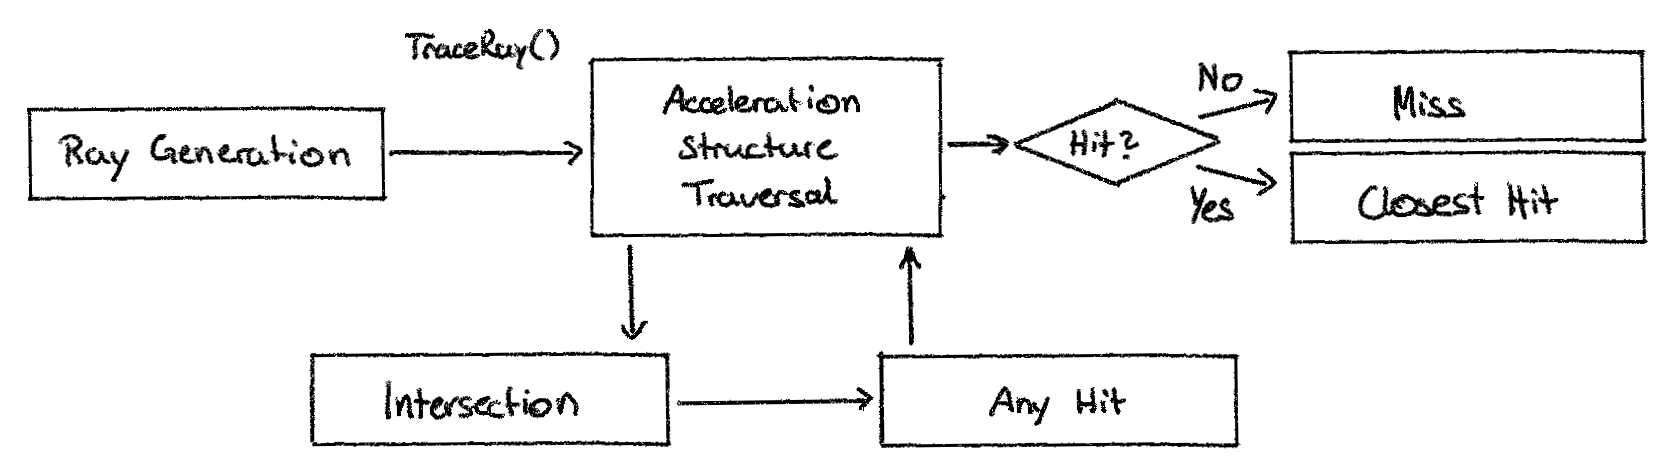
\includegraphics[width=\textwidth]{optix-kernel.png}
    \end{center}
    \caption{optix pipeline \cite{nvidia_nvidia_2022}}
    \label{fig:optix-kernel}
\end{figure}

The \textit{Ray Generation} program is the entry point of the device execution.
One uses a particular host code function to initiate the device-sided execution.
From here on, one can call additional functions to build an execution sequence.

A \textit{Intersection} and \textit{Bounds} program are necessary for the acceleration structure.
If one calls the trace function, it iterates through the data structure until the routine reaches a leaf.
For custom geometric primitives, one must specify the bounds and intersection programs so that OptiX knows how to process them during iteration.
The only exceptions are triangles and curves since they are already predefined.
OWL forms, on top of it, an abstraction for minimum expenditure.

The last two required programs are the \textit{Closest Hit} and \textit{Miss} program.
Both describe a case each, whether a ray has hit an object or not.
The execution of these programs starts after a complete iteration through the acceleration structure. 
After the execution, the application returns to the trace function call.
The only distinction between the two is that the data from the hit object is available in the closest hit program.

\section{Application Design}

This section intends to give a general overview of the application.
It describes the individual tasks of the application.
One will walk through some essential points that shaped the application design.
Note that the decision was based on simplicity and not necessarily robust and flexible design.

Let one start with a host-only functionality, which is loading mesh and material data.
Three-dimensional meshes have different representations and need corresponding loaders to bring the vertex normal and position data to memory.
Besides that, these representations can also contain information about the material data.
Accordingly, large libraries can load any file format for objects.
However, this seemed to be convoluted, and thus one decided to use an OBJ loader because of its simplicity. 
Another argument for the OBJ format was that all object vertices are in global coordinates; if needed, one could also load the normals and UV data.
One described the materials of the objects via a JSON format.

The next consideration is the exchange of data and where the data should be made available.
OptiX offers for the exchange of data two strategies.
The first is the so-called SBT or shader binding table.
They allow the programmer to bind specific data to a program of the OptiX pipeline.
An essential difference to the second option is that the data will be only available to the designated program.
The second option is to create global constants that make the data available everywhere in the device.
However, the only important attribute is simplicity and creating a global constant containing any data required during the renderer's lifetime is the easiest choice.

The next point is the path tracing itself, especially if one selects a recursive or iterative approach for path tracing.
Depending on the chosen strategy, the tasks of the programmes look different, i.e. the implementation of the path tracer is in \textit{Closest Hit}  or \textit{Ray Generation} program.
Intuitively, a recursive approach would be the most straightforward approach because one described path tracing as a recursive formula.
However, one chooses an iterative version because the path construction is more apparent, and the procedure is easier to understand.
Hence, the implementation will be in the \textit{Ray Generation} program.

One summarises the different decisions and draws the connection to how these interoperate in the application.
The host-sided application loads all required data for the tracer, initialises with OWL the OptiX components and uploads the data to the graphics card.
Afterwards, one launches the path tracing, and the host waits until the result is available through a host device buffer.
The launch causes an invocation of the \textit{Ray Generation} program per pixel, which controls the calculation of paths that have a vertex on the camera plane associated with the corresponding pixel.
The \textit{Closest Hit} and \textit{Miss} programs set the necessary state that allows the tracer to load the mesh data in the path tracing routine.
After the device has finished all calculations, the host can read the result and write it to a predefined destination. 

The last parts of this chapter explain essential aspects of the path tracer in more detail and provide a language-agnostic pseudocode.
\section{Path Construction Routine}

\section{Disney Evaluation Routines}

\section{Disney Sampling Routine}
